\documentclass[letterpaper,10pt]{article}
\usepackage[utf8]{inputenc}
\usepackage{amsmath}
\usepackage{tikz}

\title{Reals, Bitvectors, Ordinals, and Ulps:\\a bit about floating point representations}
\author{Bill Zorn}

\begin{document}

\maketitle

\begin{abstract}
 Floating point number representations are complicated; we seek to provide a crisp definition of the terms in the title and the relationships between them. Traditionally, floating point numbers are thought of as representing the values of real numbers. In some situations, we find that it makes more sense to impose an ordering on them and treat them like signed integer ordinals, for example when computing units in the last place difference (ulps), or the Posix \texttt{nextafter()} function. We formalize the mathematical underpinnings of these relationships as operations on bitvectors.
\end{abstract}

\section{Introduction}

Floating point is tricky to get right. The idea is simple: represent real numbers with a discrete representation (such as bitvectors) that can be stored and manipulated by a computer. However, the implementation tends to be complex. Sometimes the difference between $\frac{4}{3}$ and 1.3333334 is unimportant, but sometimes it is the difference between the right answer and the wrong answer, or between SAT and UNSAT. The problem is that while they represent familiar, continuous real numbers, their discrete representation makes floating point numbers incredibly specific. If you really want the right answer, you have to be precise down to the last bit. And for most people, a vector of bits like \texttt{0b00111111101010101010101010101011} is much less intuitive to think about than the real (rational, even) number $\frac{4}{3}$.

The purpose of this text is to write down in a convient place, once and for all, the meaning of floating point numbers, and formalize the conversions between various bitvector representations that are compatible with the IEEE 754-2008 standard \cite{ieee754-2008} but general enough to be useful in other applications, for example when devising constraints for SMT solvers. This way, the author (and any other interested implementers) can avoid the trouble of having to write all this down again, or risk getting a bit of it wrong.

\section{Notation}

In order to be as general as possible, we will try to express relationships and algorithms as simple (integer or real) arithmetic rather than pseudocode which might be more ambiguous to interpret or port to a particular programming language. Since we are often working with bitvectors, it is essential that we define a formal bitvector arithmetic as well.

We treat a bitvector as a nonempty zero-indexed array of bits that each are 0 or 1. We write bitvectors out as the prefix \texttt{0b} followed by the contents of the array, from most significant to least significant. A bitvector has size $n$ equal to the number of bits in the array, which must be at least one. The least significant bit is assigned index 0, and the most significant is assigned index $n-1$.

Bitvectors support the following operations: getting the size, conversion to and from integers, indexing, concatenation and extraction, shifting left and right, and comparison for equality. Every bitvector has a fixed size: $size(\texttt{0b1}) = 1$, while $size(\texttt{0b01}) = 2$. Conversion to and from integers is straightforward and follows the typical binary representation of integers. $uint$ is an unsigned conversion, such that $uint(\texttt{0b101}) = 5$, while $sint$ is a two's complement signed conversion, such that $sint(\texttt{0b101}) = -3$. Conversion the other way is accomplished with a $bv$ constructor, which takes any positive or negative integer value as its first argument and an integer size greater than 0 as its second argument, and returns a bitvector that holds the typical two's complement binary representation of the value, masked to the appropriate size: $bv(1, 2) = \texttt{0b01}$, $bv(-1, 2) = \texttt{0b11} = bv(3, 2)$, and $bv(4, 2) = \texttt{0b00}$.

Indexing is written out using square brackets, and always yields 0 or 1: $\texttt{0b01}[0] = 1$, while $\texttt{0b01}[1] = 0$. Concatenation simply joins two bitvectors together, with the first argument being placed in the more significant bits of the output: $concat(\texttt{0b01}, \texttt{0b101}) = \texttt{0b01101}$. The syntax for extraction is slightly more complex. The first two arguments are the start and end indices, both inclusive, with the first argument being the more significant (i.e. larger). Extraction yields a new bitvector with the bits between these indices: $extract(3, 2, \texttt{0b01101}) = \texttt{0b11}$. For a bitvector $x$ of size $n$, $extract(n-1, 0, x) = x$ is the identity operation, while for all indices $0 \leq i < n$, $uint(extract(i, i, x)) = x[i]$; the application of $uint$ is necessary because extraction yields a bitvector while standard indexing yields an integer.

Shifting is written infix with the right argument always being an integer. An arithmetic right shift is written as $\texttt{>>}$, while a logical one is $\texttt{>>>}$: $\texttt{0b1101} \;\texttt{>>}\; 1 = \texttt{0b1110}$, $\texttt{0b1101} \;\texttt{>>>}\; 1 = \texttt{0b0110}$, and $\texttt{0b1101} \;\texttt{<<}\; 1 = \texttt{0b1010}$. Shifts greater than the size are handled normally; they just produce uninteresting results such as $\texttt{0b1101} \;\texttt{>>}\; 8 = \texttt{0b1111}$ and $\texttt{0b1101} \;\texttt{<<}\; 257 = \texttt{0b0000}$. Comparison is only for equality (or inequality), and only allowed between bitvectors of the same size. To determine ordering, bitvectors can be converted to the appropriate integer representation.

These conventions should translate naturally to most languages and efficient representations, such as C integers. The concatenation and extraction semantics are motivated by and identical to those used in the Rosette language \cite{rosette}.

\section{Reals as Bitvectors}

A floating point number is a triple of three things: a sign $s$, an exponent $e$, and a significand $c$. $s$ is either 0 or 1 and $e$ is a positive or negative integer. We would like $c$ to represent a fractional value; to do this, we can make it a positive integer and keep around some notion of precision $p$ which records the number of digits in $c$, as represented in a base $b$. The real value represented by a number in this representation is given in Equation \ref{eq:real}.

\begin{align} \label{eq:real}
 real(s, e, c, b, p) = (-1)^s \times b^e \times (c \times b^{1 - p})
\end{align}

For lack of another widely supported alternative, we will specialize our discussion here to the IEEE 754 (binary) standard. We fix $b = 2$, and commit to representing $c$ as a bitvector $C$ of size $p$. As we can see in Equation \ref{eq:real2}, this eliminates the extra terms $b$ and $p$ so that our representation is really a triple.

\begin{align} \label{eq:real2}
 real(s, e, C) = (-1)^s \times 2^e \times (uint(C) \times 2^{1 - size(C)})
\end{align}

The IEEE 754 assigns some floating point numbers to represent values other than finite real numbers. Specifically, numbers with greater than some ``maximum'' $e$ and $c = 0$ represent infinite real numbers of the appropriate sign, and numbers with greater than this ``maximum'' $e$ but $c \neq 0$ represent something that is not a real number, or NaN, such as the indeterminate result of $\frac{0}{0}$. If we commit to representing $e$ as a bitvector $E$ of size $w$, then this ``maximum'' value is $e_{max} = 2^{w-1} - 1$, the largest positive integer a bitvector of size $w$ can represent using a two's complement representation. Instead of using two's complement directly, the IEEE 754 standard specifies a biased representation, defining also a minimum exponent $e_{min} = 1 - e_{max}$ and $e = max(uint(E) - e_{max}, e_{min})$.

Since the values of $e$ and $c$ are already represented as bitvectors, we might as well put $s$ in a 1-bit vector $S$ with $s = uint(S)$. We fully specify the meaning of our mapping from triples of bitvectors to finite real numbers (or one of two infinite real numbers, or a symbol representing something other than a real number) in Equation \ref{eq:real3},

\begin{align} \label{eq:real3}
 real(S, E, C) =
 \begin{cases}
  NaN                                           & e > e_{max} \land c \neq 0 \\
  (-1)^s \times \infty                          & e > e_{max} \land c = 0    \\
  (-1)^s \times 2^e \times (c \times 2^{1 - p}) & e \leq e_{max}
 \end{cases}
\end{align}
where:
\begin{description}
 \item $w = size(E)$
 \item $p = size(C)$
 \item $e_{max} = 2^{w-1} - 1$
 \item $e_{min} = 1 - e_{max}$
 \item $s = uint(S)$
 \item $e = max(uint(E) - e_{max}, e_{min})$
 \item $c = uint(C)$.
\end{description}

Let us call this the explicit triple of bitvectors or ``explicit triple'' representation of a floating point number. Except for its neglect of the distinction between quiet and signaling NaNs, this formulation agrees completely with IEEE 754, assuming the ability to identify the correct bitvectors $S$, $E$, and $C$. However, this representation is not as compact: as presented in Equation \ref{eq:real3}, some real numbers can be represented in multiple ways. For example, the triple $(\texttt{0b0}, \texttt{0b01}, \texttt{0b10})$ represents $(-1)^0 \times 2^0 \times (2 \times 2^{-1}) = 1$. But so does $(\texttt{0b0}, \texttt{0b10}, \texttt{0b01})$, as $(-1)^0 \times 2^1 \times (1 \times 2^{-1}) = 1$ as well. Similarly, having $E$ as 0 or 1 gives an equivalent $e = e_{min}$ due to the max in the definition of $e$. And there are $2 \times (2^w - 1)$ ways to represent 0.

Any real number representable with $e > e_{min}$ and $C[p-1] = 0$ (i.e. the high bit of $C$ is 0, or $c < 2^{p-1}$) can be similarly represented by shifting $C$ 1 bit to the left and subtracting 1 from $e$. Thus each representable number has a canonical representation, where either $C[p-1] = 1$, or $e = e_{min}$. To take advantage of this, the IEEE 754 standard records the high bit of $C$ implicitly as the otherwise unused case where $E$ is 0, and keeps track of the rest of $C$ as a shorter bitvector $T$ of size $p - 1$.

The mapping from IEEE 754 bitvectors to reals is given in Equation \ref{eq:real4},

\begin{align} \label{eq:real4}
 real(S, E, T) =
 \begin{cases}
  NaN                                                         & e' > e_{max} \land c \neq 0  \\
  (-1)^s \times \infty                                        & e' > e_{max} \land c = 0     \\
  (-1)^s \times 2^{e'} \times ((c' + 2^{p-1}) \times 2^{1-p}) & e_{min} \leq e' \leq e_{max} \\
  (-1)^s \times 2^{e_{min}} \times (c' \times 2^{1 - p})      & e' < e_{min}
 \end{cases}
\end{align}
where:
\begin{description}
 \item $w = size(E)$
 \item $p = size(T) + 1$
 \item $e_{max} = 2^{w-1} - 1$
 \item $e_{min} = 1 - e_{max}$
 \item $s = uint(S)$
 \item $e' = uint(E) - e_{max}$
 \item $c' = uint(T)$.
\end{description}

Let us call this the implicit triple of bitvectors, or ``implicit triple'' or ``IEEE 754 triple'' representation of floating point numbers. We also say that the IEEE binary interchange format uses a ``packed bitvector'' or ``implicit packed'' or just ``packed'' representation $B = concat(S, E, T)$. $S$ can always be recovered, and $E$ and $T$ can be recovered as long as $w$ or $p$ is known. 

This formulation is equivalent to the description in section 3.4 of \cite{ieee754-2008}. For clarity, we have tried to name our terms according to similar concepts from the IEEE 754 standard, distinguishing $e'$ and $c'$ because they are not necessarily the exact exponent or fractional value. The treatment here should not differ materially from the IEEE 754 standard, and is intended mostly to provide Equations \ref{eq:real3} and \ref{eq:real4} and their requisite definitions in a compact form.

Converting between the explicit and implicit representations is surprisingly tricky. When going from implicit to explicit, all we need to do is find the correct value of the implicit bit to concatenate with $T$. Usually, this is can be determined by checking if $uint(E) == 0$, but we also need to be careful not to concatenate $\texttt{0b1}$ to an infinity and turn it into NaN. The complete formula is given in Equation \ref{eq:conv1},

\begin{align} \label{eq:conv1}
 explicit(S, E, T) =
 \begin{cases}
  (S, E, concat(\texttt{0b0}, T)) & uint(E) = 0 \; \lor                   \\
                                  & (uint(E) = 2^w - 1 \land uint(T) = 0) \\
  (S, E, concat(\texttt{0b1}, T)) & \text{else}
 \end{cases}
\end{align}
where:
\begin{description}
 \item $w = size(E)$.
\end{description}

Going the other way, from the explicit to the implicit representation, is more complicated. First, we need to be able to put an explicitly represented floating point number in canonical form. One technique for doing this is expressed in Equation \ref{eq:canon},

\begin{align} \label{eq:canon}
 canonicalize(S, E, C) =
 \begin{cases}
  (S, E, C)                                             & e > e_{max} \\
  (S, bv(0, w), C)                                      & c = 0       \\
  (S, bv(0, w), C \;\texttt{<<}\: x                     & h < z       \\
  (S, bv(e - offset + e_{max}, w), C \;\texttt{<<}\: x) & \text{else}
 \end{cases}
\end{align}
where:
\begin{description}
 \item $w = size(E)$
 \item $e_{max} = 2^{w-1} - 1$
 \item $e_{min} = 1 - e_{max}$
 \item $e = max(uint(E) - e_{max}, e_{min})$
 \item $c = uint(C)$
 \item $z = clz(C)$
 \item $h = e - e_{min}$
 \item $x = min(z, h)$.
\end{description}

Note the use of $clz$, or ``count leading zeros'', which counts the number of zeros in the most significant bits of a bitvector before the most significant 1 (or the total number of bits, if all are 0). This is not generally considered a primitive operation in bitvector arithmetic, but it can be implemented efficiently for bitvectors of known size. $x$ is the largest offset we can shift by, to either ensure that $C[p-1] = 1$ or that $e = e_{min}$. Note also that for all floating point numbers that do not represent finite real numbers, i.e. infinities and NaNs, canonicalization is a no-op, as we need to be careful not to convert infinities to NaNs or vice versa and we have no mapping to real numbers to inform any changes to our representations of NaNs.

With the ability to canonicalize our explicit representation, we can now convert it to the implicit representation used by IEEE 754. Given a canonical explicit representation, we can usually just chop off the most significant (implicit) bit of $C$ to produce the appropriate $T$. There is still one problematic edge case, when we have a NaN where only the most significant bit of $C$ is 1, as simply chopping that bit off will yield an infinity. To avoid this, we preserve the 1 in the most significant bit of $T$; this loses some information, but that is unavoidable anyway since there are more explicit NaNs due to the extra bit in $C$.

Fortunately the conversion doesn't lose any information about representions of real numbers. This is why we use the perhaps odd-looking max in the definition $e = max(uint(E) - e_{max}, e_{min})$. We could just as well allow $e = -e_{max}$ in the explicit representation and represent more real numbers closer to zero, but this would cause another edge case in the conversion because those numbers would not be representable with the implicit representation. The explicit to implicit conversion is given in Equation \ref{eq:conv2},

\begin{align} \label{eq:conv2}
 implicit(S, E, C) =
 \begin{cases}
  (S_c, E_c, bv(1,p-1) \;\texttt{<<}\; (p-2)) & uint(E_c) = 2^w - 1 \; \land \\
                                             & uint(C_c) \neq 0 \; \land    \\
                                             & uint(T') = 0                  \\
  (S_c, E_c, T') & \text{else}
 \end{cases}
\end{align}
where:
\begin{description}
 \item $(S_c, E_c, C_c) = canonicalize(S, E, C)$
 \item $w = size(E_c)$
 \item $p = size(C_c$
 \item $T' = extract(p-2, 0, C_c)$.
\end{description}

Often when discussing floating point representations, much ado is made about ``subnormal'' or ``denormalized'' numbers. We have neglected to discuss them at all, because in our formalization they can be treated the same as any other number. A subnormal number is simply a floating point number with minimum exponent $e = e_{min}$ and a 0 in the high (implicit) bit of $C$. By definition, any such number can have only one representation (unless it representes 0). These numbers are important because they close the gap between the smallest number that can be represented with $C[p-1] = 1$ and 0 in a uniform way, as shown in \ref{idonthaveafigure}. Their existence explains the strange contortions we go through defining the relationship between $E$ and $e$; once we accept those contortions, their real value at least is easy to specify.

It should be noted that most hardware implementations use the packed bitvector representation; i.e. on a typical implementation using 32-bit single-precision floats, $\frac{4}{3}$ would be represented as 
\begin{align*}
 \texttt{0b00111111101010101010101010101011} \text{,}
\end{align*}
which would unpack (assuming $w=8$, $p=24$) to the implicit triple 
\begin{align*}
 (\texttt{0b0}, \texttt{0b01111111}, \texttt{0b01010101010101010101011})
\end{align*}
or the explicit triple 
\begin{align*}
 (\texttt{0b0}, \texttt{0b01111111}, \texttt{0b101010101010101010101011}) \text{.}
\end{align*}
The floating point theory defined as part of the SMT-LIB standard specifies floating point literals in a form equivalent to the implicit triple representation, i.e. the term of sort \texttt{(\_ FloatingPoint 8 24)}, where 8 and 24 are $w$ and $p$ respectively, that represents the real number closest to $\frac{4}{3}$, is written 
\begin{align*}
 \texttt{(fp \#b0 \#b01111111 \#b01010101010101010101011)} \text{.}
\end{align*}

We should also comment briefly on the possible sizes of bitvectors that can be used in these representations. We require that $size(S) = 1$, $size(E) = w \geq 2$, and $size(C) = size(T) + 1 = p \geq 2$. Since a bitvector has to have at least one bit in our notation, the restriction on $p$ is obvious. The restriction on $w$ is due to issues that arise with the max-based definition of $e$ failing to properly distinguish between infinity and zero when $e_{min} = 0$, and could be lifted with the appropriate special cases.

\section{Reals as Bitvectors as Ordinals}

Floating point numbers represent real numbers, but since they do so with bitvectors, they have some properties that bear more resemblance to integers. For example, it might be more important to know how close two real values $r_1$ and $r_2$ are, not in terms of their real difference $r_2 - r_1$, but in terms of the number of representable floating point numbers that exist between them. This quantity, typically referred to as as units in the last place, or ``ulps,'' is entirely dependent on the properties of the floating point representation in question and independent of the properties of real numbers.

To compute ulps, it can be helpful to think of floating point numbers as ordinals. By ``ordinals,'' we mean integers that impose a total ordering on all real values representable with a given floating point representation, not true ordinal numbers in the mathematical sense. A similar notion is presented in the IEEE 754 standard's totalOrder predicate. The floating point numbers of a given representation with finite $w$ and $p$ form a finite set, so a total ordering is possible, and indeed that is what totalOrder provides. However that ordering has some properties that might be surprising: all of the NaNs are ordered, which is necessary for a total ordering but perhaps not helpful, and more problematically -0.0 is less than +0.0, even though both have the same real value.

Several different orderings are possible: we choose one that is hopefully the least surprising for implementers, and discuss how it compares to the totalOrder predicate and other alternatives. We implement this ordering with a function $ord(F)$, which takes a floating point number $F$ in some known representation (such as a packed bitvector or implicit triple with known $w$ and $p$) and produces a positive or negative integer. We would like $ord(F)$ to have the following properties:

\begin{enumerate}
 \item If $real(F) = 0.0$, $ord(F) = 0$. I.e. all floating point numbers that represent a real value of zero (including ones that have a negative sign) have an order of 0.
 \item If $real(F_1) = real(F_2)$, then $ord(F_1) = ord(F_2)$. I.e. floating point numbers that represent the same real value have the same order.
 \item If $real(F_1) < real(F_2)$, then $ord(F_1) < ord(F_2)$. I.e. floating point numbers are ordered by their real value.
 \item If $real(F_1) = -\infty$ and $real(F_2) = \infty$, then $ord(F_2) - ord(F_1)$ is equal to the number of distinct real values the representation can represent (including the two infinities, but not including any NaNs) minus one. I.e. the ordinals are tightly packed: there is no positive $i$ such that there is no $F$ that has $ord(F)$ and yet there is some $F'$ that has $ord(F') > i$, or analogously for negative $i$.
 \item If $real(F)$ is NaN, then $ord(F)$ is undefined. In general, the order of a floating point number that represents NaN cannot be relied upon to be meaningful, so the safest thing to do is refuse to assign it meaning. An implementation might want to do something in this case like return an error, or extend the notion of an ordinal to include NaN and return that. In some situations there might be implementation-specific meaning, which we will discuss in more detail later.
\end{enumerate}

To help visualize, we can draw a floating point representation out on a number line, as in Figures \ref{fig:numberline1} and \ref{fig:numberline2}. Each tick on the line indicates a representable floating point number $F$, with $real(F)$ printed above the line and $ord(F)$ below it. Positive and negative 0 overlap, and share an order of 0. We draw the NaNs somewhere past the infinities, just as a reminder of their existence; they have no meaningful position on the number line. In Figure \ref{fig:numberline1}, we distribute the numbers according to their real value, while in Figure \ref{fig:numberline1} we distribute them evenly, more in accordance with their order or their properties as bitvectors.

\begin{figure}[t!]
 \centering
 \caption{Floating point numbers with $w=2$, $p=2$, distributed by real value.} \label{fig:numberline1}
 \smallskip
 \centering
 \resizebox{\textwidth}{!}{
 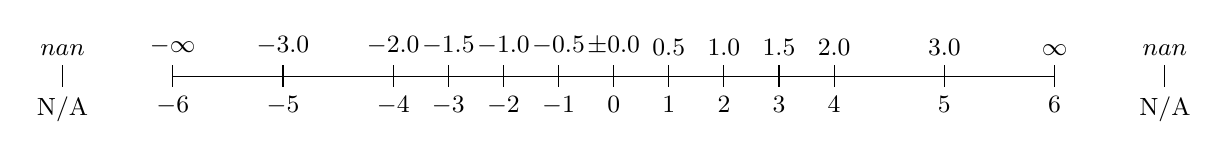
\begin{tikzpicture}[scale= 7.0/5.0]
  \draw (-4,0) -- (4,0);
   \foreach \i/\o/\r in {0.0/0/\pm0.0,0.5/1/0.5,1.0/2/1.0,1.5/3/1.5,2.0/4/2.0,3.0/5/3.0,4.0/6/\infty,5.0/\text{N/A}/nan,-0.5/-1/-0.5,-1.0/-2/-1.0,-1.5/-3/-1.5,-2.0/-4/-2.0,-3.0/-5/-3.0,-4.0/-6/-\infty,-5.0/\text{N/A}/nan}
   {
    \draw (\i,0.1) -- + (0,-0.2) node[below] {\small $\o$} + (0,0.0) node[above] {\small $\r$};
   }
    \end{tikzpicture}
 }
\end{figure}

\begin{figure}[t!]
 \centering
 \caption{Floating point numbers with $w=2$, $p=2$, distributed uniformly.} \label{fig:numberline2}
 \smallskip
 \resizebox{\textwidth}{!}{
 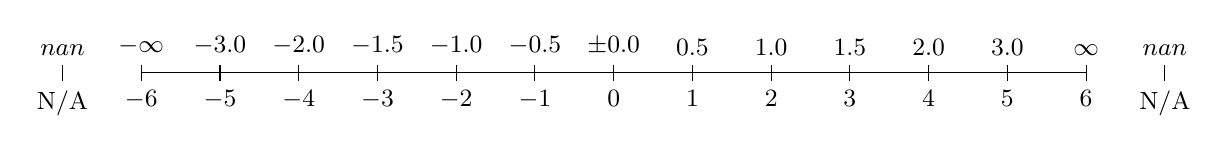
\begin{tikzpicture}[scale=1.0]
  \draw (-6,0) -- (6,0);
   \foreach \i/\o/\r in {0/0/\pm0.0,1/1/0.5,2/2/1.0,3/3/1.5,4/4/2.0,5/5/3.0,6/6/\infty,7/\text{N/A}/nan,-1/-1/-0.5,-2/-2/-1.0,-3/-3/-1.5,-4/-4/-2.0,-5/-5/-3.0,-6/-6/-\infty,-7/\text{N/A}/nan}
   {
    \draw (\i,0.1) -- + (0,-0.2) node[below] {\small $\o$} + (0,0.0) node[above] {\small $\r$};
   }
    \end{tikzpicture}
 }
\end{figure}

We can implement $ord(F)$ using arithmetic. The computation for implicit triples is given in Equation \ref{eq:ord1},

\begin{align} \label{eq:ord1}
 ord(S, E, T) = 
 \begin{cases}
  undefined       & u > umax\\
  (-1)^s \times u & u \leq umax
 \end{cases}
\end{align}
where:
\begin{description}
 \item $w = size(E)$
 \item $p = size(T) + 1$
 \item $umax = (2^w-1) \times 2^{p-1}$
 \item $s = uint(S)$
 \item $u = (uint(E) \times 2^{p-1}) + uint(T)$.
\end{description}

The new quatities $u$ and $umax$ represent the absolute value of the order and the maximum defined order, or the order of $\infty$, respectively.

\begin{align} \label{eq:ord2}
 ord(S, E, C) = 
 \begin{cases}
  undefined                                     & v = vmax \land c > 0\\
  (-1)^s \times umax                            & v = vmax \land c = 0
 \end{cases}
\end{align}
where:
\begin{description}
 \item $w = size(E)$
 \item $p = size(C)$
 \item $umax = (2^w-1) \times 2^{p-1}$
 \item $vmax = 2^w - 1$
 \item $s = uint(S)$
 \item $v = uint(E)$
 \item $c = uint(C)$.
\end{description}

Interestingly, it is much easier to compute for the implicit triple representation, as the canonical bitvectors are ordered in a convenient way.

\bibliographystyle{ieeetr}
\bibliography{ref}

\end{document}
